% Phase 4 -- written by Abdullah
% Every number comes from a file under results/ or from src/baseline_cnn.py.
\section{Phase 4: Training, Evaluation and Bias Check}

\subsection{Baseline CNN design}
The baseline is a small convolutional network trained from scratch
(\texttt{src/baseline\_cnn.py}, class \texttt{BaselineCNN}). It is the
reference point for the pretrained EfficientNet-B0. It takes a
$3 \times 224 \times 224$ image and returns 14 logits (no softmax inside the
model). It has four convolution blocks, each made of a $3 \times 3$
convolution (padding 1), batch normalisation, ReLU and $2 \times 2$ max
pooling, with 32, 64, 128 and 256 channels. Global average pooling,
dropout ($0.3$) and one linear layer follow. The model has
\textbf{392,974} trainable parameters.

\begin{table}[H]
  \centering
  \begin{tabular}{|l|l|r|}
    \hline
    \textbf{Layer} & \textbf{Output size} & \textbf{Parameters} \\ \hline
    Input & $3 \times 224 \times 224$ & 0 \\ \hline
    Conv 3$\to$32 + BatchNorm + ReLU & $32 \times 224 \times 224$ & 960 \\ \hline
    MaxPool 2 & $32 \times 112 \times 112$ & 0 \\ \hline
    Conv 32$\to$64 + BatchNorm + ReLU & $64 \times 112 \times 112$ & 18,624 \\ \hline
    MaxPool 2 & $64 \times 56 \times 56$ & 0 \\ \hline
    Conv 64$\to$128 + BatchNorm + ReLU & $128 \times 56 \times 56$ & 74,112 \\ \hline
    MaxPool 2 & $128 \times 28 \times 28$ & 0 \\ \hline
    Conv 128$\to$256 + BatchNorm + ReLU & $256 \times 28 \times 28$ & 295,680 \\ \hline
    MaxPool 2 & $256 \times 14 \times 14$ & 0 \\ \hline
    Global average pooling & $256$ & 0 \\ \hline
    Dropout (0.3) & $256$ & 0 \\ \hline
    Linear 256$\to$14 & $14$ logits & 3,598 \\ \hline
    \textbf{Total} & & \textbf{392,974} \\ \hline
  \end{tabular}
  \caption{Baseline CNN layers. Parameter counts include the batch-norm
  weights and biases.}
\end{table}

\begin{figure}[H]
  \centering
  \begin{tikzpicture}[
      font=\scriptsize,
      box/.style={draw, rounded corners, align=center, minimum height=1.0cm, minimum width=2.1cm, inner sep=3pt},
      arr/.style={-{Latex}, thick}
    ]
    \node[box] (in) {Input\\$3 \times 224 \times 224$};
    \node[box, right=0.4cm of in] (b1) {Block 1\\Conv 32\\BN, ReLU, Pool};
    \node[box, right=0.4cm of b1] (b2) {Block 2\\Conv 64\\BN, ReLU, Pool};
    \node[box, right=0.4cm of b2] (b3) {Block 3\\Conv 128\\BN, ReLU, Pool};
    \node[box, right=0.4cm of b3] (b4) {Block 4\\Conv 256\\BN, ReLU, Pool};
    \node[box, below=1.3cm of in] (gap) {Global avg.\\pool (256)};
    \node[box, right=0.4cm of gap] (drop) {Dropout\\0.3};
    \node[box, right=0.4cm of drop] (fc) {Linear\\14 logits};
    \draw[arr] (in) -- (b1);
    \draw[arr] (b1) -- (b2);
    \draw[arr] (b2) -- (b3);
    \draw[arr] (b3) -- (b4);
    \draw[arr] (b4.south) -- ++(0,-0.5) -| (gap.north);
    \draw[arr] (gap) -- (drop);
    \draw[arr] (drop) -- (fc);
  \end{tikzpicture}
  \caption{Baseline CNN block diagram (\texttt{src/baseline\_cnn.py}).}
\end{figure}

The loss is cross-entropy with label smoothing $0.1$. The optimiser is
AdamW with a cosine-annealing learning-rate schedule. These are the same
settings as for EfficientNet, because both models use the shared trainer
\texttt{src/train.py}.

\subsection{Baseline hyperparameters}
The baseline was trained \textbf{once} with fixed values. It was not tuned.
The EfficientNet hyperparameter search is described in Phase 3.

\begin{table}[H]
  \centering
  \begin{tabular}{|l|l|p{7.2cm}|}
    \hline
    \textbf{Hyperparameter} & \textbf{Value} & \textbf{Justification} \\ \hline
    Learning rate & $1 \times 10^{-3}$ & Usual AdamW starting value for training a small CNN from scratch. \\ \hline
    Batch size & 32 & Fits comfortably on a Colab T4 GPU and gives stable batch-norm statistics. \\ \hline
    Dropout & 0.3 & Moderate regularisation before the single linear layer. \\ \hline
    Weight decay & $1 \times 10^{-4}$ & Light L2-style regularisation; same value as the EfficientNet runs. \\ \hline
    Label smoothing & 0.1 & Reduces over-confidence on noisy scraped labels; same as EfficientNet. \\ \hline
    Epochs run & 20 (maximum 20) & Early stopping (patience 5) did not trigger; the cosine schedule was set for 20 epochs. \\ \hline
  \end{tabular}
  \caption{Baseline hyperparameters. Training command:
  \texttt{python src/train.py --model baseline --epochs 20 --batch-size 32
  --lr 1e-3 --weight-decay 1e-4 --label-smoothing 0.1 --num-workers 2}.}
\end{table}

\subsection{Validation strategy}
We use the 70/15/15 stratified train/validation/test split made in Phase 2
(seed 42), which gives 2,986 training, 640 validation and 641 test images.
The validation set is used during training for early stopping and for
choosing the best checkpoint. The test set is used once, at the end, to
produce the predictions evaluated below. We did not use K-fold
cross-validation: the held-out test set is fixed from Phase 2, and
repeated training of the EfficientNet model would be costly.

\subsection{Training curves}
Figure~\ref{fig:curves-baseline} shows the baseline's loss and accuracy per
epoch. Over the 20 epochs the validation loss fell to $1.7605$ and
validation accuracy rose to $0.5422$, while training accuracy reached
$0.5271$ (\texttt{results/history\_baseline.csv}). Both curves were still
improving at epoch 20, so the baseline is probably under-trained; with
fixed settings and a single run we did not train it for longer. Training
accuracy stays close to validation accuracy, so there is no strong sign
of over-fitting.

\begin{figure}[H]
  \centering
  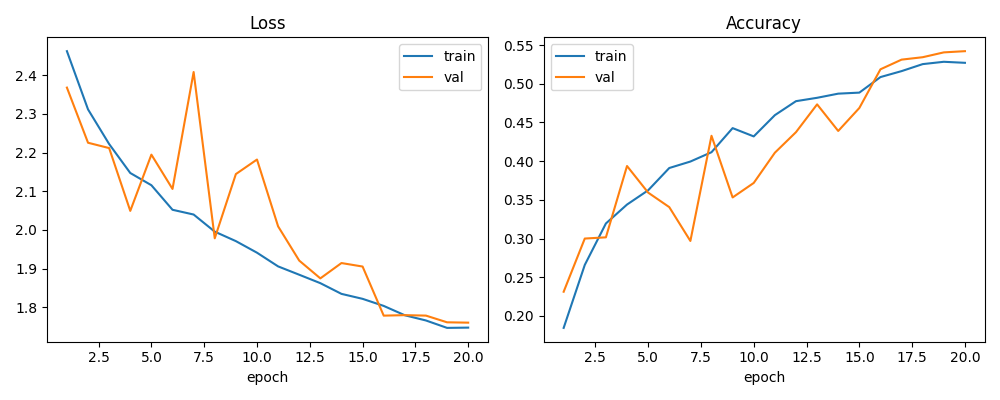
\includegraphics[width=0.9\textwidth]{curves_baseline.png}
  \caption{Baseline CNN training and validation curves.}
  \label{fig:curves-baseline}
\end{figure}

Figure~\ref{fig:curves-efficientnet} shows the EfficientNet-B0 curves.
\textbf{TODO:} add one or two sentences on these curves from
\texttt{results/history\_efficientnet.csv}.

\begin{figure}[H]
  \centering
  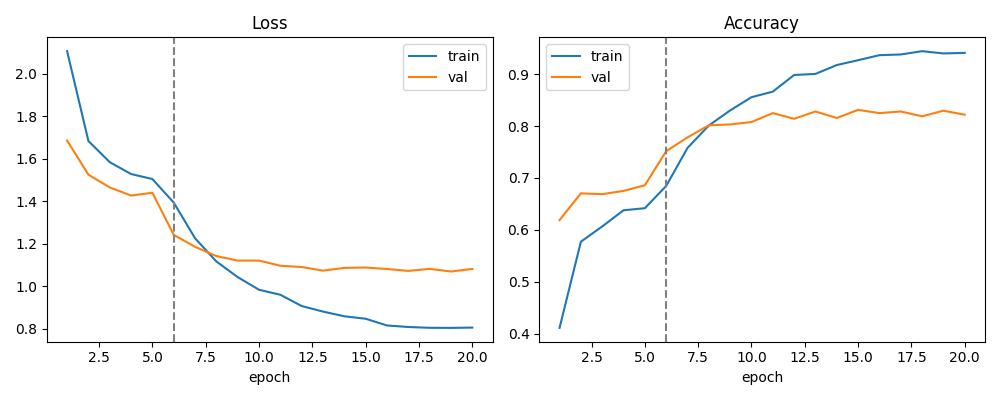
\includegraphics[width=0.9\textwidth]{curves_efficientnet.png}
  \caption{EfficientNet-B0 training and validation curves.}
  \label{fig:curves-efficientnet}
\end{figure}

% Summary:
% 1) Describes the from-scratch baseline CNN: layer table, block diagram, loss and optimiser.
% 2) Lists the fixed baseline hyperparameters with a short reason each, and the 70/15/15 split.
% 3) Shows both training-curve figures, with baseline numbers taken from history_baseline.csv.